\documentclass[12pt]{article}
\usepackage[right=1.25in,left=1.25in,top=1.1in,bottom=1.1in]{geometry}
\usepackage{hyperref}
\hypersetup{colorlinks, citecolor=blue, filecolor=blue, linkcolor=blue, urlcolor=blue}
\usepackage{graphicx}
\usepackage{epstopdf}
\usepackage{url}
%\usepackage[round]{natbib}
\usepackage[
    backend=biber,
    style=bwl-FU,
    url=false,
    doi=false,
    eprint=false,
    natbib=true
]{biblatex}
\addbibresource{reference.bib}
\usepackage{amsmath,amsthm} 
\usepackage{engord}
\usepackage{float}
\usepackage{subfig}
\usepackage{pdflscape}
\usepackage{booktabs}
\usepackage{pgfplots}
\usepackage{adjustbox}
\usepackage{dcolumn}
\newcolumntype{.}{D{.}{.}{-1}}
\usepackage{blindtext}
\pgfplotsset{compat=1.14}
\pgfplotsset{every axis label/.append style={font=\tiny}}
\usepackage[labelsep=period]{caption} 
\usepackage{amssymb} 
\usepackage{multirow} 
\usepackage{xr}
\usepackage{setspace}
\onehalfspacing
\usepackage{sectsty}
\sectionfont{\large}
\subsectionfont{\normalsize}
\subsubsectionfont{\normalsize}
\newcommand{\specialcell}[2][c]{\begin{tabular}[#1]{@{}l@{}}#2\end{tabular}}

%%%%%%%%%%%%%%%%%%%%%%%%%%%%%%%%%%%%%%%%%%%%%%%%%%%%%%%%%%%%%
\begin{document} 
\title{\begin {figure}[H]
\centering

\includegraphics[width=9cm]{badge.png}
\end {figure}\vspace*{2.5cm} \hspace*{-0.5cm} \\\textbf{Digital Tools for Finance\\\vspace{5mm} \\Markowitz-Optimal Portfolio Under Inflation in China}}
\author{Yunpeng Zhang\and Zhiying Hu\and Xuanzhi Lin
\and Zelong Han}
\date{\vspace{5mm} December 18, 2022}
\maketitle
\thispagestyle{empty}

\clearpage
\tableofcontents
\setcounter{page}{1}

\clearpage

\setcounter{page}{1}

\section{Introduction}
Global inflation has reached its highest level since 2008 in recent years due to the shock of covid-19, supply chain disruptions, and increasingly tense international conditions. More than half of the countries with inflation-targeting frameworks have already exceeded their target rates. For many households around the world, rising inflation poses a significant challenge. What's more, for a long period, China's economic growth has been overly dependent on government investment, bank credit, and currency issuance. Coupled with the lack of a tight monitoring mechanism, rapid economic growth has been accompanied by the risk of inflation.\\
Inflation implies a prolonged period of rising price levels, which leads to a contraction in the real value of assets. The erosion of the real return of a portfolio caused by inflation is one of the fundamental risks faced by investors in financial markets. Therefore, it is of great theoretical and practical significance to study the inflation-hedging ability of various types of assets and to construct investment portfolios under inflation consideration.\\
Related research focuses on two main areas. One is to study the relationship between asset returns and inflation and to test the ability of various types of assets to hedge inflation. In general, real estate is an ideal investment tool for storing value \citep{FAMA1977115,di2012can}, while stocks do not provide an effective inflation hedge\citep{rapach2002long,engsted2002relation}, and gold has a good value preservation function only in the long term \citep{levin2006short}. The second is to study the asset allocation strategy under inflation risk. In terms of asset selection, equities dominate, bonds, commodities, and derivatives (including swaps, options, and spots) are included, and some scholars also cover real estate and collectibles \citep{attie2009inflation}. In terms of model construction, basically follow Markowitz's mean-variance model \citep{qin2004optimal, yu2015study}.\\
In this paper, we construct an inflation-hedging portfolio based on the assessment of the inflation-hedging ability of four types o assets. The second part analyzes the inflation-hedging ability of Chinese financial assets; the third part constructs an inflation-hedging portfolio, and the fourth part concludes.\\

\section{The Examination of the Inflation Hedging Ability of the Financial Asset in China}
\subsection{Model Construction}
We divide the nominal return into three parts: real return rate, expected inflation rate, and unexpected inflation rate following the method in \citep{yu2015study}.\\
\begin{equation}
E(R_{t}|\Omega_{t-1})=E(r_{t}|\Omega_{t-1})+\beta E(\pi_{t}|\Omega_{t-1})+\gamma \left [\pi_{t}-E(\pi_{t}|\Omega_{t-1})  \right ] \label{equation1}
\end{equation}
where $E(R_{t}|\Omega_{t-1}$ is the nominal expected return, $E(r_{t}|\Omega_{t-1})$ is the real expected return, $E(\pi_{t}|\Omega_{t-1})$ is the expected inflation rate of time $t$, and $\pi_{t}-E(\pi_{t}|\Omega_{t-1})$ is the unexpected inflation rate of time $t$.\\
Based on Formula \eqref{equation1}, the model can be rewritten as
\begin{equation}
R_{t}=\alpha +\beta E(\pi_{t}|\Omega_{t-1})+\gamma \left [\pi_{t}-E(\pi_{t}|\Omega_{t-1})  \right ]+\eta _{t}
\label{equation2}
\end{equation}
where $R_{t}$ the nominal return is the dependent variable, $E(\pi_{t}|\Omega_{t-1})$ the expected inflation rate, and $\pi_{t}-E(\pi_{t}|\Omega_{t-1})$ the unexpected inflation rate are the independent variables. $\alpha$, $\beta$ and $\gamma$ are estimated parameters, and $\eta _{t}$ is the error term.\\
$\beta$ measures the hedging ability against expected inflation, and the $\gamma$ measure the hedging ability against unexpected inflation. If these two parameters are less than zero, the asset has a negative hedging ability against expected and unexpected inflation, if they are in the interval of zero, the asset has a partial hedging ability and if they are larger than 1, the asset has an excess hedging ability. If $\beta$ and $\gamma$ are equal to zero, there is no hedging ability, and if $\beta$ and $\gamma$ are equal to one, the asset is fully hedged against the risk of inflation.\\
\subsection{Data}
The sample period is from January 2010 to December 2021 except for the real estate data. Due to the lack of availability of the data, the sample period of real estate price data is from June 2011 to December 2021. All data got from Choice.\\
To eliminate the non-stationary time series data, all assets' returns take the form of monthly year-on-year logarithms. To be specific, the return is calculated by$$return_{t}=log(\frac{price_{t}}{price_{t-12}})=log(price_{t})-log(price_{t-12})$$. \\
To be consistent, the real inflation rate is expressed in the logarithmic form of the monthly year-on-year CPI data.\\
The expected inflation rate at time t is represented by the one-year national bond's yield to maturity at time t-1. And the unexpected inflation rate is the difference between the real inflation rate and the expected inflation rate.\\
We choose four types of assets to do the examination, including commodity futures, real estate, spot gold, and Hushen 300 industry index.\\
For commodity futures, we choose sixteen kinds of future contracts from the Shanghai and Dalian futures exchange: Soybeans No. 1, soybeans No. 2, yellow corn, LLDPE, soybean meal, palm oil, soybean oil, PVC, cathode copper, aluminum, zinc, gold, natural rubber, fuel oil, rebar and wire rod. We downloaded the settlement price at the end of each month to calculate returns.\\
The spot gold price is the monthly closing price of gold T+D published by the Shanghai Gold Exchange.\\
As for the stock market data, we selected the monthly closing prices of the Hushen 300 industry index, which includes energy, raw materials, industry, optional consumption, the main consumption, medicine and health care, finance and real estate, information technology, the utility and the telecommunication service.\\
We also selected monthly data on residential prices in Tier 1, Tier 2, and Tier 3 cities.\\
\subsection{Empirical Results}
Adopting Formula \eqref{equation2}, we do the regression of all four kinds of assets to test their hedging abilities.\\

\subsubsection{Commodity Futures}
The regression results of commodity futures are shown in Table \ref{cf1} - \ref{cf4}. \\

\begin{table}[!htbp] \centering 
  \caption{The inflation hedging ability of commodity futures} 
  \label{cf1} 
\begin{tabular}{@{\extracolsep{5pt}}lD{.}{.}{-3} D{.}{.}{-3} D{.}{.}{-3} D{.}{.}{-3} } 
\\[-1.8ex]\hline 
\hline \\[-1.8ex] 
 & \multicolumn{4}{c}{\textit{Dependent variable:}} \\ 
\cline{2-5} 
\\[-1.8ex] & \multicolumn{4}{c}{commodity futures} \\ 
\\[-1.8ex] & \multicolumn{1}{c}{Soybeans No.1} & \multicolumn{1}{c}{Soybeans No.2} & \multicolumn{1}{c}{Yellow Corn} & \multicolumn{1}{c}{LLDPE}\\
\hline \\[-1.8ex] 
 expected\_inflation & -5.983^{***} & -8.515^{***} & 4.295^{*} & -1.201 \\ 
  & (2.063) & (2.253) & (2.480) & (2.207) \\ 
  & & & & \\ 
 unexpected\_inflation & 0.280 & 1.704^{*} & 0.928 & -2.303^{**} \\ 
  & (0.876) & (0.957) & (1.053) & (0.937) \\ 
  & & & & \\ 
 Constant & 0.205^{***} & 0.251^{***} & -0.078 & 0.012 \\ 
  & (0.057) & (0.062) & (0.068) & (0.061) \\ 
  & & & & \\ 
\hline \\[-1.8ex] 
Observations & \multicolumn{1}{c}{144} & \multicolumn{1}{c}{144} & \multicolumn{1}{c}{144} & \multicolumn{1}{c}{144} \\ 
R$^{2}$ & \multicolumn{1}{c}{0.071} & \multicolumn{1}{c}{0.157} & \multicolumn{1}{c}{0.021} & \multicolumn{1}{c}{0.042} \\ 
Adjusted R$^{2}$ & \multicolumn{1}{c}{0.058} & \multicolumn{1}{c}{0.145} & \multicolumn{1}{c}{0.007} & \multicolumn{1}{c}{0.029} \\ 
Residual Std. Error & \multicolumn{1}{c}{0.138} & \multicolumn{1}{c}{0.151} & \multicolumn{1}{c}{0.166} & \multicolumn{1}{c}{0.148} \\ 
F Statistic & \multicolumn{1}{c}{5.366$^{***}$} & \multicolumn{1}{c}{13.119$^{***}$} & \multicolumn{1}{c}{1.530} & \multicolumn{1}{c}{3.103$^{**}$} \\ 
\hline 
\hline \\[-1.8ex] 
\textit{Note:}  & \multicolumn{4}{r}{$^{*}$p$<$0.1; $^{**}$p$<$0.05; $^{***}$p$<$0.01} \\ 
\end{tabular} 
\end{table} 

\begin{table}[!htbp] \centering 
  \caption{The inflation hedging ability of commodity futures} 
  \label{cf2} 
\begin{tabular}{@{\extracolsep{5pt}}lD{.}{.}{-3} D{.}{.}{-3} D{.}{.}{-3} D{.}{.}{-3} } 
\\[-1.8ex]\hline 
\hline \\[-1.8ex] 
 & \multicolumn{4}{c}{\textit{Dependent variable:}} \\ 
\cline{2-5} 
\\[-1.8ex] & \multicolumn{4}{c}{commodity futures} \\ 
\\[-1.8ex] & \multicolumn{1}{c}{Soybean Meal} & \multicolumn{1}{c}{Palm Oil} & \multicolumn{1}{c}{Soybean Oil} & \multicolumn{1}{c}{PVC}\\
\hline \\[-1.8ex] 
 expected\_inflation & -2.744 & -9.813^{***} & -10.418^{***} & -5.093^{**} \\ 
  & (2.186) & (2.878) & (2.420) & (2.575) \\ 
  & & & & \\ 
 unexpected\_inflation & 0.616 & 2.774^{**} & 2.056^{**} & -2.176^{**} \\ 
  & (0.928) & (1.222) & (1.028) & (1.042) \\ 
  & & & & \\ 
 Constant & 0.094 & 0.302^{***} & 0.311^{***} & 0.152^{**} \\ 
  & (0.060) & (0.079) & (0.067) & (0.072) \\ 
  & & & & \\ 
\hline \\[-1.8ex] 
Observations & \multicolumn{1}{c}{144} & \multicolumn{1}{c}{144} & \multicolumn{1}{c}{144} & \multicolumn{1}{c}{140} \\ 
R$^{2}$ & \multicolumn{1}{c}{0.021} & \multicolumn{1}{c}{0.157} & \multicolumn{1}{c}{0.193} & \multicolumn{1}{c}{0.043} \\ 
Adjusted R$^{2}$ & \multicolumn{1}{c}{0.007} & \multicolumn{1}{c}{0.145} & \multicolumn{1}{c}{0.182} & \multicolumn{1}{c}{0.029} \\ 
Residual Std. Error & \multicolumn{1}{c}{0.146} & \multicolumn{1}{c}{0.193} & \multicolumn{1}{c}{0.162} & \multicolumn{1}{c}{0.164} \\ 
F Statistic & \multicolumn{1}{c}{1.540} & \multicolumn{1}{c}{13.171$^{***}$} & \multicolumn{1}{c}{16.912$^{***}$} & \multicolumn{1}{c}{3.049$^{*}$} \\ 
\hline 
\hline \\[-1.8ex] 
\textit{Note:}  & \multicolumn{4}{r}{$^{*}$p$<$0.1; $^{**}$p$<$0.05; $^{***}$p$<$0.01} \\ 
\end{tabular} 
\end{table} 

\begin{table}[!htbp] \centering 
  \caption{The inflation hedging ability of commodity futures} 
  \label{cf3} 
\begin{tabular}{@{\extracolsep{5pt}}lD{.}{.}{-3} D{.}{.}{-3} D{.}{.}{-3} D{.}{.}{-3} } 
\\[-1.8ex]\hline 
\hline \\[-1.8ex] 
 & \multicolumn{4}{c}{\textit{Dependent variable:}} \\ 
\cline{2-5} 
\\[-1.8ex] & \multicolumn{4}{c}{commodity futures} \\ 
\\[-1.8ex] & \multicolumn{1}{c}{Cathode Copper} & \multicolumn{1}{c}{Aluminum} & \multicolumn{1}{c}{Zinc} & \multicolumn{1}{c}{Gold}\\
\hline \\[-1.8ex] 
 expected\_inflation & -7.728^{**} & -4.968^{**} & -4.505 & -7.502^{***} \\ 
  & (3.181) & (2.188) & (2.936) & (1.733) \\ 
  & & & & \\ 
 unexpected\_inflation & -1.291 & -1.685^{*} & -5.235^{***} & 5.103^{***} \\ 
  & (1.351) & (0.929) & (1.247) & (0.736) \\ 
  & & & & \\ 
 Constant & 0.251^{***} & 0.157^{***} & 0.145^{*} & 0.269^{***} \\ 
  & (0.087) & (0.060) & (0.081) & (0.048) \\ 
  & & & & \\ 
\hline \\[-1.8ex] 
Observations & \multicolumn{1}{c}{144} & \multicolumn{1}{c}{144} & \multicolumn{1}{c}{144} & \multicolumn{1}{c}{144} \\ 
R$^{2}$ & \multicolumn{1}{c}{0.040} & \multicolumn{1}{c}{0.042} & \multicolumn{1}{c}{0.111} & \multicolumn{1}{c}{0.425} \\ 
Adjusted R$^{2}$ & \multicolumn{1}{c}{0.027} & \multicolumn{1}{c}{0.029} & \multicolumn{1}{c}{0.098} & \multicolumn{1}{c}{0.417} \\ 
Residual Std. Error & \multicolumn{1}{c}{0.213} & \multicolumn{1}{c}{0.146} & \multicolumn{1}{c}{0.196} & \multicolumn{1}{c}{0.116} \\ 
F Statistic & \multicolumn{1}{c}{2.952$^{*}$} & \multicolumn{1}{c}{3.113$^{**}$} & \multicolumn{1}{c}{8.806$^{***}$} & \multicolumn{1}{c}{52.096$^{***}$} \\ 
\hline 
\hline \\[-1.8ex] 
\textit{Note:}  & \multicolumn{4}{r}{$^{*}$p$<$0.1; $^{**}$p$<$0.05; $^{***}$p$<$0.01} \\ 
\end{tabular} 
\end{table} 

\begin{table}[!htbp] \centering 
  \caption{The inflation hedging ability of commodity futures} 
  \label{cf4} 
\begin{tabular}{@{\extracolsep{5pt}}lD{.}{.}{-3} D{.}{.}{-3} D{.}{.}{-3} D{.}{.}{-3} } 
\\[-1.8ex]\hline 
\hline \\[-1.8ex] 
 & \multicolumn{4}{c}{\textit{Dependent variable:}} \\ 
\cline{2-5} 
\\[-1.8ex] & \multicolumn{4}{c}{commodity futures} \\ 
\\[-1.8ex] & \multicolumn{1}{c}{Natural Rubber} & \multicolumn{1}{c}{Fuel Oil} & \multicolumn{1}{c}{Rebar} & \multicolumn{1}{c}{Wire Rod}\\
\hline \\[-1.8ex] 
 expected\_inflation & -14.338^{***} & -4.748 & -2.444 & 0.377 \\ 
  & (3.966) & (4.215) & (3.704) & (3.346) \\ 
  & & & & \\ 
 unexpected\_inflation & 3.739^{**} & -1.961 & -1.508 & -0.351 \\ 
  & (1.685) & (1.790) & (1.535) & (1.387) \\ 
  & & & & \\ 
 Constant & 0.392^{***} & 0.095 & 0.080 & 0.015 \\ 
  & (0.109) & (0.116) & (0.102) & (0.093) \\ 
  & & & & \\ 
\hline \\[-1.8ex] 
Observations & \multicolumn{1}{c}{144} & \multicolumn{1}{c}{144} & \multicolumn{1}{c}{142} & \multicolumn{1}{c}{140} \\ 
R$^{2}$ & \multicolumn{1}{c}{0.166} & \multicolumn{1}{c}{0.013} & \multicolumn{1}{c}{0.008} & \multicolumn{1}{c}{0.001} \\ 
Adjusted R$^{2}$ & \multicolumn{1}{c}{0.154} & \multicolumn{1}{c}{-0.001} & \multicolumn{1}{c}{-0.007} & \multicolumn{1}{c}{-0.014} \\ 
Residual Std. Error & \multicolumn{1}{c}{0.265} & \multicolumn{1}{c}{0.282} & \multicolumn{1}{c}{0.241} & \multicolumn{1}{c}{0.218} \\ 
F Statistic & \multicolumn{1}{c}{14.007$^{***}$} & \multicolumn{1}{c}{0.897} & \multicolumn{1}{c}{0.533} & \multicolumn{1}{c}{0.057} \\ 
\hline 
\hline \\[-1.8ex] 
\textit{Note:}  & \multicolumn{4}{r}{$^{*}$p$<$0.1; $^{**}$p$<$0.05; $^{***}$p$<$0.01} \\ 
\end{tabular} 
\end{table}

Combining the results in four tables, commodity futures are better at hedging expected inflation risk and less good at hedging unanticipated inflation risk in general. Specifically speaking, in the 1\% level, the $\beta$ of Soybeans No.1, Soybeans No.2, Palm Oil, Soybean Oil, Gold, Natural Rubber, and the $\gamma$ of Zinc, Gold are significantly different from zero. In the 5\% level, the $\beta$ of PVC, Cathode Copper, Aluminum, and the $\gamma$ of LLDPE, Palm Oil, Soybean Oil, PVC, and Natural Rubber are significantly different from zero. In the 10\% level, the $\beta$ of Yellow Corn, and the $\gamma$ of Soybeans No.2 and Aluminum are significantly different from zero. However, the estimated parameters of Soybean Meal, Fuel Oil, Rebar, and Wire Rod are not significant.\\

\subsubsection{Gold}
\begin{table}[!htbp] \centering 
  \caption{The inflation hedging effect of spot gold} 
  \label{gold} 
\begin{tabular}{@{\extracolsep{5pt}}lD{.}{.}{-3} } 
\\[-1.8ex]\hline 
\hline \\[-1.8ex] 
 & \multicolumn{1}{c}{\textit{Dependent variable:}} \\ 
\cline{2-2} 
\\[-1.8ex] & \multicolumn{1}{c}{Spot Gold} \\ 
\hline \\[-1.8ex] 
 expected\_inflation & -7.454^{***} \\ 
  & (1.714) \\ 
  & \\ 
 unexpected\_inflation & 5.128^{***} \\ 
  & (0.728) \\ 
  & \\ 
 Constant & 0.267^{***} \\ 
  & (0.047) \\ 
  & \\ 
\hline \\[-1.8ex] 
Observations & \multicolumn{1}{c}{144} \\ 
R$^{2}$ & \multicolumn{1}{c}{0.431} \\ 
Adjusted R$^{2}$ & \multicolumn{1}{c}{0.423} \\ 
Residual Std. Error & \multicolumn{1}{c}{0.115} \\ 
F Statistic & \multicolumn{1}{c}{53.374$^{***}$} \\ 
\hline 
\hline \\[-1.8ex] 
\textit{Note:}  & \multicolumn{1}{r}{$^{*}$p$<$0.1; $^{**}$p$<$0.05; $^{***}$p$<$0.01} \\ 
\end{tabular} 
\end{table} 
From table \ref{gold}, the estimated parameters $\beta$ and $\gamma$ are significant at the 1\% level. Based on the result, we could say that spot gold has a negative hedging effect against expected inflation and an excess hedging effect against unexpected inflation.\\

\subsubsection{Industry Stocks}
The regression results of industry stocks are shown in Table \ref{stock1} - \ref{stock2}. \\
\begin{table}[!htbp] \centering 
  \caption{The inflation hedging ability of industry stocks} 
  \label{stock1} 
\begin{adjustbox}{center}
\begin{tabular}{@{\extracolsep{5pt}}lD{.}{.}{-3} D{.}{.}{-3} D{.}{.}{-3} D{.}{.}{-3} D{.}{.}{-3} } 
\\[-1.8ex]\hline 
\hline \\[-1.8ex] 
 & \multicolumn{5}{c}{\textit{Dependent variable:}} \\ 
\cline{2-6} 
\\[-1.8ex] & \multicolumn{5}{c}{industry stocks} \\ 
\\[-1.8ex] & \multicolumn{1}{c}{Energy} & \multicolumn{1}{c}{Material} & \multicolumn{1}{c}{Industry} & \multicolumn{1}{c}{Optional} & \multicolumn{1}{c}{Main}\\ 
\hline \\[-1.8ex] 
 expected\_inflation & -2.188 & -9.063^{**} & -7.416 & -3.864 & -4.955 \\ 
  & (3.515) & (4.328) & (4.488) & (3.589) & (3.551) \\ 
  & & & & & \\ 
 unexpected\_inflation & -2.023 & -6.328^{***} & -6.728^{***} & -5.326^{***} & -1.565 \\ 
  & (1.493) & (1.838) & (1.907) & (1.525) & (1.509) \\ 
  & & & & & \\ 
 Constant & -0.017 & 0.250^{**} & 0.206^{*} & 0.169^{*} & 0.300^{***} \\ 
  & (0.097) & (0.119) & (0.123) & (0.099) & (0.098) \\ 
  & & & & & \\ 
\hline \\[-1.8ex] 
Observations & \multicolumn{1}{c}{144} & \multicolumn{1}{c}{144} & \multicolumn{1}{c}{144} & \multicolumn{1}{c}{144} & \multicolumn{1}{c}{144} \\ 
R$^{2}$ & \multicolumn{1}{c}{0.013} & \multicolumn{1}{c}{0.082} & \multicolumn{1}{c}{0.082} & \multicolumn{1}{c}{0.080} & \multicolumn{1}{c}{0.016} \\ 
Adjusted R$^{2}$ & \multicolumn{1}{c}{-0.001} & \multicolumn{1}{c}{0.069} & \multicolumn{1}{c}{0.069} & \multicolumn{1}{c}{0.067} & \multicolumn{1}{c}{0.002} \\ 
Residual Std. Error & \multicolumn{1}{c}{0.235} & \multicolumn{1}{c}{0.290} & \multicolumn{1}{c}{0.300} & \multicolumn{1}{c}{0.240} & \multicolumn{1}{c}{0.238} \\ 
F Statistic & \multicolumn{1}{c}{0.925} & \multicolumn{1}{c}{6.296$^{***}$} & \multicolumn{1}{c}{6.287$^{***}$} & \multicolumn{1}{c}{6.134$^{***}$} & \multicolumn{1}{c}{1.126} \\ 
\hline 
\hline \\[-1.8ex] 
\textit{Note:}  & \multicolumn{5}{r}{$^{*}$p$<$0.1; $^{**}$p$<$0.05; $^{***}$p$<$0.01} \\ 
\end{tabular} 
\end{adjustbox}
\end{table} 

\begin{table}\centering
  \caption{The inflation hedging ability of industry stocks} 
  \label{stock2} 
\begin{adjustbox}{center}
\begin{tabular}{@{\extracolsep{5pt}}lD{.}{.}{-3} D{.}{.}{-3} D{.}{.}{-3} D{.}{.}{-3} D{.}{.}{-3} } 
\\[-1.8ex]\hline 
\hline \\[-1.8ex] 
 & \multicolumn{5}{c}{\textit{Dependent variable:}} \\ 
\cline{2-6} 
\\[-1.8ex] & \multicolumn{5}{c}{industry stocks} \\ 
\\[-1.8ex] & \multicolumn{1}{c}{Medicine} & \multicolumn{1}{c}{Finance} & \multicolumn{1}{c}{Info} & \multicolumn{1}{c}{Tele} & \multicolumn{1}{c}{Utility}\\ 
\hline \\[-1.8ex] 
 expected\_inflation & -11.363^{***} & -2.650 & -6.993^{*} & 4.802 & -4.069 \\ 
  & (3.302) & (3.117) & (4.168) & (4.398) & (3.401) \\ 
  & & & & & \\ 
 unexpected\_inflation & -4.228^{***} & -5.384^{***} & -2.201 & -1.412 & -7.689^{***} \\ 
  & (1.403) & (1.324) & (1.770) & (1.868) & (1.445) \\ 
  & & & & & \\ 
 Constant & 0.416^{***} & 0.090 & 0.253^{**} & -0.135 & 0.085 \\ 
  & (0.091) & (0.086) & (0.115) & (0.121) & (0.094) \\ 
  & & & & & \\ 
\hline \\[-1.8ex] 
Observations & \multicolumn{1}{c}{144} & \multicolumn{1}{c}{144} & \multicolumn{1}{c}{144} & \multicolumn{1}{c}{144} & \multicolumn{1}{c}{144} \\ 
R$^{2}$ & \multicolumn{1}{c}{0.098} & \multicolumn{1}{c}{0.108} & \multicolumn{1}{c}{0.023} & \multicolumn{1}{c}{0.019} & \multicolumn{1}{c}{0.171} \\ 
Adjusted R$^{2}$ & \multicolumn{1}{c}{0.085} & \multicolumn{1}{c}{0.095} & \multicolumn{1}{c}{0.009} & \multicolumn{1}{c}{0.005} & \multicolumn{1}{c}{0.159} \\ 
Residual Std. Error & \multicolumn{1}{c}{0.221} & \multicolumn{1}{c}{0.208} & \multicolumn{1}{c}{0.279} & \multicolumn{1}{c}{0.294} & \multicolumn{1}{c}{0.228} \\ 
F Statistic & \multicolumn{1}{c}{7.641$^{***}$} & \multicolumn{1}{c}{8.541$^{***}$} & \multicolumn{1}{c}{1.625} & \multicolumn{1}{c}{1.390} & \multicolumn{1}{c}{14.542$^{***}$} \\ 
\hline 
\hline \\[-1.8ex] 
\textit{Note:}  & \multicolumn{5}{r}{$^{*}$p$<$0.1; $^{**}$p$<$0.05; $^{***}$p$<$0.01} \\ 
\end{tabular} 
\end{adjustbox}
\end{table}

\newpage
Combining the results in table \ref{stock1} and table \ref{stock2}, the industry stock indexes are having a negative hedging effect on both expected and unexpected inflation risk in general. Specifically speaking, in the 1\% level, the $\gamma$ of Raw Material, Industry, Optional Consumption, Medicine and Health Care, Finance and Real Estate, and Utility are significantly different from zero. Meanwhile, in the 1\% level, the $\beta$ of Medicine and Health Care is significantly different from zero. In the 5\% level, the $\beta$ of Raw Material is significantly different from zero. In the 10\% level, the $\beta$ of Information technology is significantly different from zero. However, the estimated parameters of Energy, Main Consumption, and Telecommunication services are not significant.\\

\subsubsection{Real Estate}
\begin{table}[!htbp] \centering 
  \caption{The inflation hedging ability of real estate} 
  \label{estate} 
\begin{tabular}{@{\extracolsep{5pt}}lD{.}{.}{-3} D{.}{.}{-3} D{.}{.}{-3} } 
\\[-1.8ex]\hline 
\hline \\[-1.8ex] 
 & \multicolumn{3}{c}{\textit{Dependent variable:}} \\ 
\cline{2-4} 
\\[-1.8ex] & \multicolumn{3}{c}{real estate} \\ 
\\[-1.8ex] & \multicolumn{1}{c}{first-tier} & \multicolumn{1}{c}{second-tier} & \multicolumn{1}{c}{third-tier}\\ 
\hline \\[-1.8ex] 
 expected\_inflation & 0.720 & 2.110^{**} & 2.589^{***} \\ 
  & (1.294) & (0.850) & (0.835) \\ 
  & & & \\ 
 unexpected\_inflation & -0.172 & 0.449 & 0.704^{*} \\ 
  & (0.568) & (0.373) & (0.367) \\ 
  & & & \\ 
 Constant & 0.046 & -0.010 & -0.030 \\ 
  & (0.036) & (0.024) & (0.023) \\ 
  & & & \\ 
\hline \\[-1.8ex] 
Observations & \multicolumn{1}{c}{127} & \multicolumn{1}{c}{127} & \multicolumn{1}{c}{127} \\ 
R$^{2}$ & \multicolumn{1}{c}{0.004} & \multicolumn{1}{c}{0.049} & \multicolumn{1}{c}{0.079} \\ 
Adjusted R$^{2}$ & \multicolumn{1}{c}{-0.012} & \multicolumn{1}{c}{0.034} & \multicolumn{1}{c}{0.064} \\ 
Residual Std. Error & \multicolumn{1}{c}{0.077} & \multicolumn{1}{c}{0.051} & \multicolumn{1}{c}{0.050} \\ 
F Statistic & \multicolumn{1}{c}{0.277} & \multicolumn{1}{c}{3.189$^{**}$} & \multicolumn{1}{c}{5.338$^{***}$} \\ 
\hline 
\hline \\[-1.8ex] 
\textit{Note:}  & \multicolumn{3}{r}{$^{*}$p$<$0.1; $^{**}$p$<$0.05; $^{***}$p$<$0.01} \\ 
\end{tabular} 
\end{table} 

The inflation hedging ability of real estate is shown in table \ref{estate}. The first-tier cities' real estate has no obvious hedging ability against inflation. The $\beta$ of the second-tier cities' real estate is significantly different from zero at the 5\% level, which means that it has an excess hedging ability against expected inflation risk. In addition, the $\beta$ of the third-tier cities' real estate is significantly different from zero at the 1\% level, and the $\gamma$ is significantly different from zero at the 10\% level. Thus, the third-tier cities' real estate has an excess hedging ability against expected inflation risk and a partial hedging ability against unexpected inflation risk.\\
\begin{table}[ht] \centering
\caption{Inflation hedging effect of the tested assets}
\label{effect}
\begin{tabular}{rll}
  \hline
  Expected Inflation & Unexpected Inflation\\ 
  \hline
  soybeans.No..1 & soybeans.No..2 \\ 
  soybeans.No..2 & LLDPE \\ 
  yellow.corn & palm.oil \\ 
  palm.oil & soybean.oil \\ 
  soybean.oil & PVC \\
  PVC & aluminum \\ 
  cathode.copper & zinc \\ 
  aluminum & gold \\ 
  gold & natural.rubber \\ 
  natural.rubber & Spot Gold \\ 
  Spot Gold & Material \\ 
  Material & Industry \\ 
  Medicine\_health\_care & Optional\_consumption \\
  Information\_technology & Medicine\_health\_care \\ 
  second.tier real estate & Finance\_and\_real\_estate \\ 
  third.tier real estate & Utility \\ 
  & third.tier real estate\\ 
   \hline
\end{tabular}
\end{table}

\newpage
\section{The Construction of Inflation Hedging Portfolio by Mean Variance Method}
\subsection{Model Construction}
Markowitz proposed the classic portfolio theory in 1952. In this essay, when constructing the optimal mean-variance portfolio, we minimize the portfolio’s volatility at the given expected return. The model can be expressed as follows:
\begin{align*}
&\min \quad \sigma_{p}^{2}=\sum_{i=1}^{n} x_{i}^{2}\sigma_{i}^{2} + \sum_{j=1,j\neq i}^{n} x_{i}x_{j}\sigma_{ij} \\
& \begin{array}{r@{\quad}l@{}l@{\quad}l}
s.t.& E(R_{p})=\sum_{i=1}^{n}E(R_{i})=X^{T}\cdot R\\
&\sum_{i=1}^{n} x_{i}=1
\end{array}
\end{align*}
where $\sigma_{p}^{2}$ is the variance of the portfolio, $x_{i}$ or $x_{j}$ represents the percentage of asset $i$ or $j$ in the portfolio, $\sigma_{i}^{2}$ is the variance of asset $i$. $E(R_{p})$ is the expected return of the portfolio, $R$ is a $N x 1$ vector consisting of the expected return of all assets, and $X$ is a $N x 1$ vector consisting of weights of all assets.\\
Based on the test results in Part 2, among the 30 kinds of assets, we exclude 8 assets from the portfolio that do not have inflation-hedging effects, including four commodity futures, Soybean Meal, Fuel Oil, Rebar, Wire Rod, three industry stocks, Energy, Main Consumption, and Telecommunication services and first-tier real estate. The remaining 22 asset returns have a significant inflation-hedging ability. Therefore, we choose these kinds of assets to construct the portfolio.\\

\subsection{Portfolio Performance}
To construct the portfolio of multiple risky assets, we give 10,000 different weights to assets to calculate the feasible portfolio. Then, we present them as mean-variance scatter plots to visualize the performance of the portfolio with different weights. It is shown in Figure \ref{fig1}.\\
\begin{figure}[H]
    \centering
    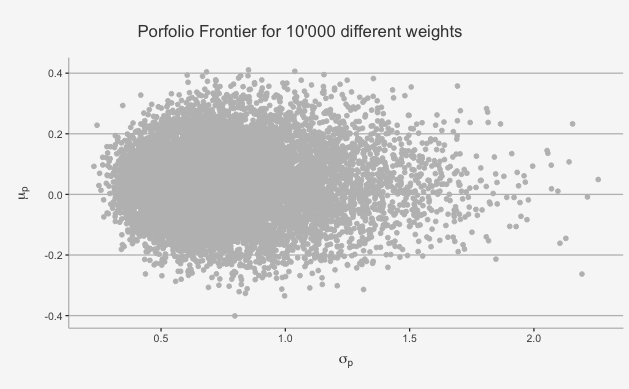
\includegraphics[width=0.8\linewidth]{feasible_port.png}
    \caption{Feasible Portfolio}
    \label{fig1}
\end{figure}
Using the formula in Section 3.1, the expected return and variance of different efficient portfolios can be calculated. Thus we can get the portfolio efficient frontier, which is shown in Figure \ref{fig2}.\\
\begin{figure}[H]
    \centering
    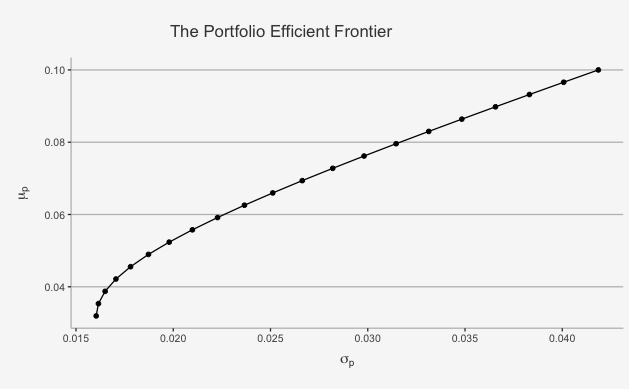
\includegraphics[width=0.8\linewidth]{EF.png}
    \caption{The portfolio efficient frontier}
    \label{fig2}
\end{figure}

In addition, the performance of the minimum-variance portfolio and the tangency portfolio is calculated, as shown in table \ref{portfolio}. The Minimum-variance portfolio has an expected return of 3.194\% and a standard deviation of 0.016, while the tangency portfolio has an expected return of 20.8\% and a standard deviation of 0.101. When focusing on the weight of different kinds of assets, real estate investment plays a pivotal role in hedging inflation risks. To achieve a higher return, investors are recommended to short real estate in third-tier cities and long real estate in second-tier cities. With no restrictions on short-selling, investors can also choose to combat inflation risk by shorting commodity futures or industry stocks that have negative hedging effects.

\begin{table}[ht]
\centering
\caption{Weights of two portfolios} 
\label{portfolio}
\begin{tabular}{rrr}
  \hline
 & Minimum\_Variance & Tangency \\ 
  \hline
soybeans.No..1 & 0.07660 & 0.09200 \\ 
  soybeans.No..2 & 0.03268 & -0.56361 \\ 
  yellow.corn & -0.03444 & -0.01810 \\ 
  LLDPE & 0.16480 & -0.46870 \\ 
  palm.oil & -0.08382 & 0.00566 \\ 
  soybean.oil & 0.23658 & 0.44568 \\ 
  PVC & -0.13073 & -0.37670 \\ 
  cathode.copper & -0.08903 & 0.43862 \\ 
  aluminum & 0.12496 & 0.94792 \\ 
  zinc & -0.01261 & -0.33503 \\ 
  gold & 0.10168 & 0.87778 \\ 
  natural.rubber & -0.11332 & -0.59461 \\ 
  Gold\_price & -0.05229 & -0.56480 \\ 
  Material\_price & -0.09654 & -0.44755 \\ 
  Industry\_price & 0.04007 & 0.66609 \\ 
  Optional\_consumption\_price & -0.02104 & 0.46472 \\ 
  Medicine\_health\_care\_price & 0.00047 & 0.67506 \\ 
  Finance\_and\_real\_estate\_price & 0.07915 & 0.20370 \\ 
  Information\_technology\_price & 0.02372 & -0.81320 \\ 
  Utility\_price & 0.10316 & -0.62516 \\ 
  second.tier real estate & 0.31774 & 4.44097 \\ 
  third.tier real estate & 0.33219 & -3.45076 \\ 
   \hline
  Return & 0.03194 & 0.20838 \\ 
  sd & 0.01604 & 0.10149 \\ 
   \hline
\end{tabular}
\end{table}

\newpage
\section{Conclusion}
Firstly, we test the inflation hedging ability of the following four categories of assets: commodity futures, industry stocks, real estate, and spot gold. The empirical regression result shows that sixteen assets have hedging ability against expected inflation, and seventeen assets have hedging ability against unexpected inflation, as shown in Table \ref{effect}.\\
Then, we construct the mean-variance model under the consideration of inflation, using the 22 assets with obvious inflation hedging ability selected by the test results before to construct the optimal portfolio and obtain the efficient frontier. We obtain the weights of each asset, expected return, and standard deviation of both the minimum portfolio and the tangency portfolio. Results in Table \ref{portfolio} show that the tangency portfolio has a better performance than the minimum variance portfolio.\\
When constructing the portfolio, we allow short selling for all categories of assets, which is a very loose assumption. Due to the current strict restrictions on short selling in China, the portfolio construction strategy is limited to some extent. If short-selling restrictions are removed in the future, the portfolio construction strategy in this paper could be a better hedge against inflation.\\
\newpage

\printbibliography

\end{document}